\section{Lecture 14: Upsampling and Downsampling}

\subsection{Discrete-Time Processing of Continuous-Time Signals}
%
Let's consider the generic workflow
%
\begin{displaymath}
  x_c(t) \longrightarrow \boxed{h_\mathrm{samp}}
  \longrightarrow x_s(t) \longrightarrow \boxed{h_\mathrm{adc}}
  \longrightarrow x_d[n] \longrightarrow \boxed{h_\mathrm{sys}}
  \longrightarrow y_d[n] \longrightarrow \boxed{h_\mathrm{dac}}
  \longrightarrow y_c(t) \,.
\end{displaymath}
%
Here, we begin with a continuous-time signal, $x_c(t)$, which is sampled
to yield a second continuous-time signal, $x_s(t)$, whose non-zero values are
spaced by $T$ in time. This signal is next converted into the discrete-time
signal, $x_d[n]$ by the ADC filter $h_\mathrm{adc}$. $x_d[n]$ is processed
by some arbitrary system filter $h_\mathrm{sys}$ to give the filtered
discrete-time signal $y_d[n]$, and finally transformed back into a
continuous-time signal by $h_\mathrm{dac}$ to yield $y_c(t)$.\\
%
In the previous lecture, we showed that for the sampling, the CTFT
of the signal $x_c(t)$, which is band-limited to $\omega_B$, is
%
\begin{displaymath}
  X_s(\omega) = \frac{1}{T}\infsum{k}X_c(\omega - k\omega_s) \,,
\end{displaymath}
%
where $\omega_s = \frac{2\pi}{T}$, with $X_s(\omega)$ is $\omega_s$-periodic.
The DTFT of $x_d[n]$ is fundamentally the same as the CTFT of $x_s(t)$, but
is scaled in the frequency to become $2\pi$-periodic. The scaling is accomplished
by the factor $\frac{2\pi}{\omega_s} = T$ (i.e. divide by $\omega_s$ to give a
period of $1$, then multiply by the new periodicity of $2\pi$), so that the
new band-limit is $\omega_b \leftarrow \omega_B T$. As such,
%
\begin{displaymath}
  X_d(\omega) = \frac{1}{T}\infsum{k}X_s\left(\omega\frac{\omega_s}{2\pi} - k\omega_s\right)
    = \frac{1}{T}\infsum{k}X_s\left(\frac{\omega - 2\pi k}{T}\right) \,,
\end{displaymath}
%
(note the independent variable is divided by the scaling factor --
for instance, $\sin(x)$ has period 1 through the variable change
$x\leftarrow 2\pi x$). We also know from the last lecture that recreating
$y_c(t)$ from $y_d[n]$ required by the final DAC is accomplished through
low-pass filtering the DTFT of $y_d[n]$,
%
\begin{displaymath}
  Y_c(\omega) = H_\mathrm{dac}(\omega)Y_d(\omega T)
  = \infsum{n} y_d[n]\sinc\left(\frac{\pi}{T}(t - nT)\right) \,.
\end{displaymath}
%
We can simply bolt all of these stages together since the output of one
stage forms the input of another,
%
\begin{align*}
  Y_c(\omega) &= H_\mathrm{dac}(\omega)Y_d(\omega T)
  = H_\mathrm{dac}(\omega)H_\mathrm{sys}(\omega T)X_d(\omega T) \\
  &= H_\mathrm{dac}(\omega)H_\mathrm{sys}(\omega T)\frac{1}{T}\infsum{k}X_c\left(\omega - \frac{2\pi k}{T}\right) \,.
\end{align*}
%
Now, if we enforce the band-limit imposed by the reconstruction filter,
$H_{\mathrm{dac}}$, such that for
$2|\omega| > \frac{2\pi}{T}, X_c(\omega) = 0$, then
%
\begin{displaymath}
  Y_c(\omega) = \left\{\begin{array}{ccl}
  H_\mathrm{sys}(\omega T)X_c(\omega) & & |\omega| < \frac{\pi}{T} \\
  0 & & \mathrm{otherwise}
  \end{array}\right. \,,
\end{displaymath}
%
since $H_\mathrm{dac}(\omega)$ is a band-pass filter. As such, the effective
continuous-time frequency response is
%
\begin{displaymath}
  Y_r(\omega) = H_{\mathrm{eff}}(\omega)X(\omega) \,,
\end{displaymath}
%
where
%
\begin{displaymath}
  H_{\mathrm{eff}}(\omega) = \left\{\begin{array}{ccl}
  H(\omega T) & & |\omega| < \frac{\pi}{T} \\
  0 & & \mathrm{otherwise}
  \end{array}\right. \,.
\end{displaymath}
%
Consequently, we can only design filters which are active when
$|\omega| < \frac{\pi}{T}$, else the reconstruction filter will remove
any effects outside of this range; if we want to make this interval wider,
then we need to change the sampling rate.\\
%
All of this can seem a little overwhelming, so the process that
we've just discussed is depicted in Figure
\ref{fig::lecture_14_filtering_continuous}. We see that in using a
discrete-time cutoff frequency of $\omega_c$, we have
effectively filtered the continuous-time signal, $x_c(t)$, with a
continuous-time low-pass filter whose cutoff frequency is $\omega_c / T$.
This is something of an interesting result, since it suggests that we need
only design a good digital filter once, and we can simply modify the sampling
rate we use to acquire the discrete-time signal to change the effective
continuous-time cutoff frequency. Naturally there are some restrictions;
the first is that the discrete-time system must be LTI, and the second is
that the sampler must be above the Nyquist rate of the input -- if we don't
sample fast enough, then aliasing will be problematic.
%
\begin{figure}[H]
  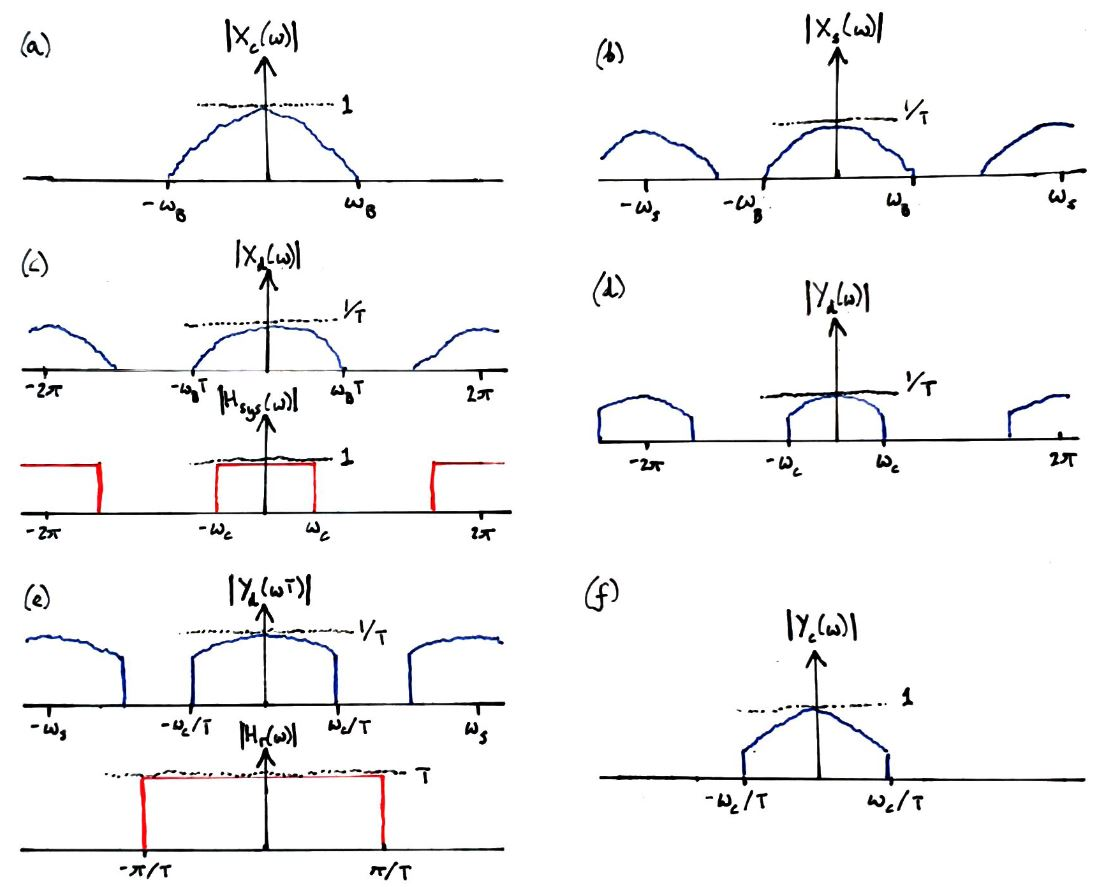
\includegraphics[width=\textwidth]{images/lecture_14_filtering_continuous.JPG}
  \caption{Filtering of a continuous-time signal with a low-pass filter.
    The CTFT of band-limited signal, $X_c(\omega)$ is shown in (a), which
    is sampled at frequency $\omega_s$ -- the CTFT of this sampled signal is
    shown in (b), and is $\omega_s$-periodic. The DTFT of the sampled signal,
    $X_d(\omega)$ is given in (c), where the band-limit becomes $\omega_B T$ and
    the spectrum is $2\pi$-periodic. Also shown in this pane is the frequency
    response of the low-pass filter, $H_\mathrm{sys}(\omega)$, with cutoff frequency
    $\omega_c$. Filtering of $X_d(\omega)$ with this filter results in $Y_d(\omega)$,
    shown in (d), the DTFT of the discrete-time signal $y_d[n]$. This spectrum is
    converted back to being $\omega_s$-periodic, yielding a modified cutoff frequency
    of $\omega_c/T$ and spectrum $Y_d(\omega T)$ in (e). Also shown in this pane is
    the low-pass filter used to remove the periodic copies in this sampled signal.
    Using this on $Y_d(\omega T)$ results in the final continuous-time signal,
    $Y_c(\omega)$, the spectrum of which is shown in pane (f), and has band-limit
    $\omega_c / T$.
  }
  \label{fig::lecture_14_filtering_continuous}
\end{figure}
%
We've been working exclusively in the frequency-domain, which raises the question
of how the impulse responses are related. Consider the continuous-time desired impulse
response, $h_\mathrm{des}(t)$. Then, the digital filter that corresponds to this
is
%
\begin{displaymath}
  h[n] = T h_\mathrm{des}(nT) \,,
\end{displaymath}
%
meaning we sample $h_\mathrm{des}(t)$ with sampling period $T$ and scale each of the
sampled values by $T$. This is referred to as \textrm{impulse invariance}, and will
be discussed in an upcoming lecture.

\subsection{Changing the Sampling Rate}
%
A common problem is that we have a signal $x[n] = x_c(nT)$, and we want to create
a second signal that is sampled at a different rate, $x^\prime[n] = x_c(nT^\prime)$,
where $T\neq T^\prime$. Assuming everything is sampled above the Nyquist rate, the
``overkill'' solution would be to reconstruct $x_c(t)$ from $x[n]$, then resample
at an appropriate rate to yield $x^\prime[n]$. While this works, we'd ideally like
a fully digital operation that doesn't need to proceed through the construction
of some analogue intermediate.

\subsubsection{Downsampling at an Integer Rate}
%
Consider the \textbf{downsampled} signal
%
\begin{displaymath}
  x_\downarrow[n] = x[nM] = x_c(nMT) \,,
\end{displaymath}
%
which takes every $M\th$ sample of some signal $x[n]$, changing the original sampling
rate of $T$ to $MT$, where $M\in\mathbb{N}$. At a system level, this can be represented
by the following block diagram:
%
\begin{displaymath}
  x[n] \longrightarrow \boxed{\downarrow M} \longrightarrow x_{\downarrow M}[n] \,.
\end{displaymath}
%
In the frequency domain, we have the DTFT of the original signal
%
\begin{displaymath}
  X(\omega) = \frac{1}{T}\infsum{k} X_c\left(\frac{\omega - 2\pi k}{T}\right) \,,
\end{displaymath}
%
where $X_c(\omega)$ is the CTFT of the original signal. The DTFT of the
downsampled signal is
%
\begin{displaymath}
  X_{\downarrow M}(\omega) = \frac{1}{T^\prime}\infsum{k} X_c\left(\frac{\omega - 2\pi k}{T^\prime}\right)
  = \frac{1}{MT}\infsum{k} X_c\left(\frac{\omega - 2\pi k}{MT}\right) \,,
\end{displaymath}
%
since $T^\prime$ is a multiple of $T$. Now, we split this summation into $M$ summations,
splitting our original summation index into the sum of two indices,
%
\begin{align*}
  X_{\downarrow M}(\omega) &= \frac{1}{M}\sum_{m=0}^{M-1}\frac{1}{T}\infsum{k^\prime}
  X_c\left(\frac{\omega - 2\pi(m + k^\prime M)}{MT}\right)
  = \frac{1}{M}\sum_{m=0}^{M-1}\left[\frac{1}{T}\infsum{k^\prime}X_c\left(
    \frac{\omega-2\pi m}{MT} - \frac{2\pi k^\prime}{T}
    \right)\right] \\
  &= \frac{1}{M}\sum_{m=0}^{M-1}X\left(\frac{\omega - 2\pi m}{M}\right)
  \,,
\end{align*}
%
where we recognise the term in square brackets as the DTFT of the continuous-time signal,
but shifted by $\frac{2\pi m}{M}$ and scaled by $M$. Then, the downsampled DTFT is
obtained by a sum of scaled and shifted copies of the original DTFT. This is precisely
what we'd expect -- the DTFT is a $2\pi$-periodic version of the CTFT, where the magnitude
of the spectrum at each point is scaled by the inverse sampling period. The final expression
in the above equation is nothing more than this; a sum of shifted versions of the original
DTFT that have been ``spread out'' by a factor of $M$ (i.e. the magnitudes of the spectral
coefficients are reduced by a factor of $M$, but the band-limit increases by a factor of
$M$. Note that the factor of $\frac{1}{M}$ on the outside of the summation compensates
for the addition of an already periodic function. This process is depicted in Figure
\ref{fig::lecture_14_downsample_alias}.
Note that the spreading out that happens as a result of the downsampling can lead to
aliasing -- the original signal would have needed to have been sampled at a minimum of $M$
times the Nyquist rate to prevent this.
%
\begin{figure}[H]
  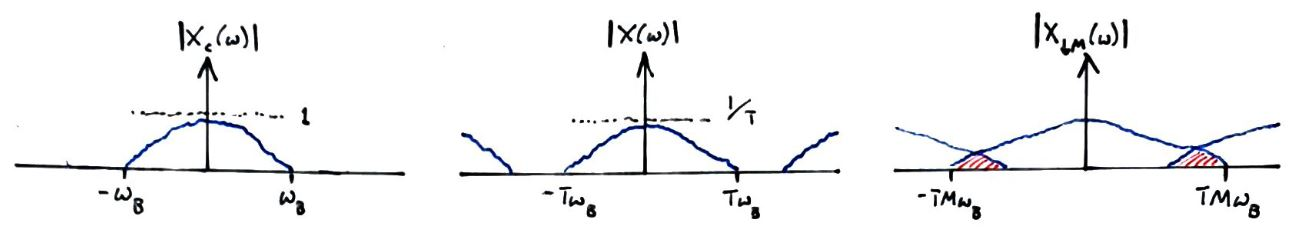
\includegraphics[width=\textwidth]{images/lecture_14_downsample_alias.JPG}
  \caption{The CTFT of the continuous-time signal, $X_c(\omega)$ and its
    discrete-time counterpart, $X(\omega)$, the latter having been acquired
    with a sampling period of $T$. Downsampling by a factor of $M$ then results
    in $X_{\downarrow M}(\omega)$, whose bandlimit is now scaled to $TM\omega_B$
    from $T\omega_B$, leading to aliasing (red hatched regions).
  }
  \label{fig::lecture_14_downsample_alias}
\end{figure}
%
\begin{exmp}
  Consider the DTFT $X(\omega) = \Lambda(2\omega/\pi)$, i.e. non-zero on the interval
  $[-\pi/2,\pi/2]$. Downsampling this by a factor of 3 results in aliasing as the
  effective band-limit becomes $3\pi/2$, consequently overlapping with copies
  (see panes (a) and (b) of Figure \ref{fig::lecture_14_triangle_example}).
  One partial solution is to low-pass filter
  the original signal, a \textbf{prefilter} such that $X^\prime(\omega)$ has band-limit
  $\pi/3$; downsampling by a factor of 3 then results in no aliasing (see panes (c) and
  (d) of Figure \ref{fig::lecture_14_triangle_example}).
  %
  \begin{figure}[H]
    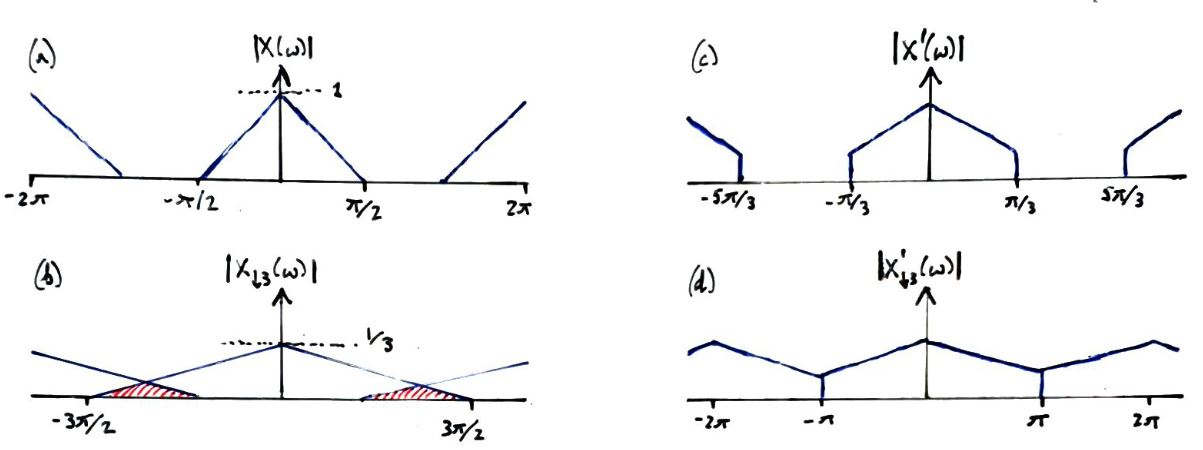
\includegraphics[width=\textwidth]{images/lecture_14_triangle_example.JPG}
    \caption{$X(\omega)$ is given in pane (a). When downsampled by a factor of
      3 (pane (b)), the signal is aliased, $X_{\downarrow 3}(\omega)$. Aliasing
      can be mitigated by first low-pass filtering the original discrete-time
      signal with cutoff frequency $\pi/3$, yielding $X^\prime(\omega)$ in
      pane (c). Downsampling of $X^\prime(\omega)$ then results in
      $X^\prime_{\downarrow 3}(\omega)$, whose band-limit is $\pi$ and does
      not overlap with periodic copies.
    }
    \label{fig::lecture_14_triangle_example}
  \end{figure}
  %
\end{exmp}
%
The previous example mentioned that low-pass filtering the original signal before
downsampling was only a partial solution; the issue is that the downsampled signal
now no longer represents the original signal due to the omission of higher frequency
components. However, if the prevention of aliasing is the primary objective, then this
cannot be avoided, and in general one needs to low-pass filter the signal with
cutoff frequency of $\pi/M$. Alternatively, if there isn't a great deal of high
frequency content in the signal, then we might be able to get away with the small
amount of aliasing that results, but this depends on how one is quantifying the
acceptable amount of aliasing.\\
%
A final scenario we'd like to emphasise is that there are situations in which one can
sample at a lower frequency than the Nyquist rate and not encounter aliasing. Consider
the band-pass spectrum in pane (a) of Figure \ref{fig::lecture_14_undersample},
which has a nominal band-limit of
$\omega_B$. Sampling at the Nyquist rate, $2\omega_B$, results in the spectrum given
in pane (b) of Figure \ref{fig::lecture_14_undersample}. However, we don't care about the
overlapping of the
two innermost regions since we can simply filter these out. Consequently, we can sample
at some other rate that is lower than the Nyquist rate, resulting in the spectrum
given in pane (c) of Figure \ref{fig::lecture_14_undersample}; the band-pass regions aren't
overlapping with anything,
and so there's no aliasing. In reality, the lowest possible sampling rate is defined more
by the non-zero bandwidth of the signal rather than its absolute band limit.
%
\begin{figure}[H]
  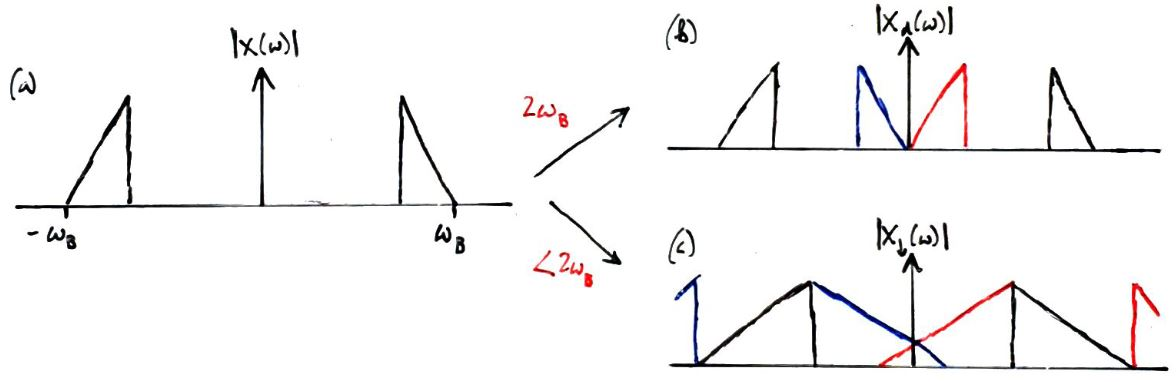
\includegraphics[width=\textwidth]{images/lecture_14_undersample.JPG}
  \caption{A qualitative example of a signal which can be downsampled below
    its Nyquist rate without aliasing. The band-limit of the signal is $\omega_B$,
    but sampling at the Nyquist rate leaves significant space between the band-pass
    regions of the spectrum and periodic copies. One can downsample below the
    Nyquist rate of the signal (pane (c)), and subsequently carve out the
    periodic copies of the spectrum, resulting in a signal which hasn't been aliased.
  }
  \label{fig::lecture_14_undersample}
\end{figure}
%

\subsubsection{Upsampling at an Integer Rate}
%
Upsampling is the process of increasing the sampling rate, resulting in more samples
than were present in the originally sampled signal, i.e.
%
\begin{displaymath}
  x_\uparrow[n] = x_c(nT/L) \,,
\end{displaymath}
%
where $L\in\mathbb{N}$. At a system level, this can be represented
by the following block diagram:
%
\begin{displaymath}
  x[n] \longrightarrow \boxed{\uparrow L} \longrightarrow x_{\uparrow L}[n] \,.
\end{displaymath}
%
The operation of an upsampler is to pad the original signal with $L-1$ zeroes
between each two samples, resulting in an intermediary signal $x_L[n]$, i.e.
%
\begin{displaymath}
  x_{L}[n] = \left\{\begin{array}{ccl}
  x[n/L] & & n = 0, \pm L, \pm 2L, \hdots \\
  0 & & \mathrm{otherwise}
  \end{array}\right. \,.
\end{displaymath}
%
However, this by itself isn't particularly helpful -- by upsampling, we'd like
to infer the signal's values at those intermediary points that we've introduced
through upsampling. To do this, we need simply pass $x_L[n]$ through a digital
low-pass filter (i.e. it's $2\pi$-periodic) with cutoff frequency $\pi/L$ and height
$L$, which we refer to as an \textrm{interpolation filter}, $H_\mathrm{int}(\omega)$.
Let's consider this mathematically. The DTFT of the zero-padded signal is
%
\begin{displaymath}
  X_L(\omega) = \infsum{n} x_L[n] \ex{-\im\omega n} = \infsum{n}x[n]\ex{-\im\omega n L}
  = X(\omega L) \,,
\end{displaymath}
%
which is the DTFT of the original signal, but compressed in the frequency axis
by a factor of $L$. This is depicted in Figure \ref{fig::lecture_14_upsample}. Note
that the low-pass filter in (c) simply carves out the $2\pi$-periodic copies of
the spectrum, returning the DTFT of the original signal but upsampled by a factor
of $L$.
%
\begin{figure}[H]
  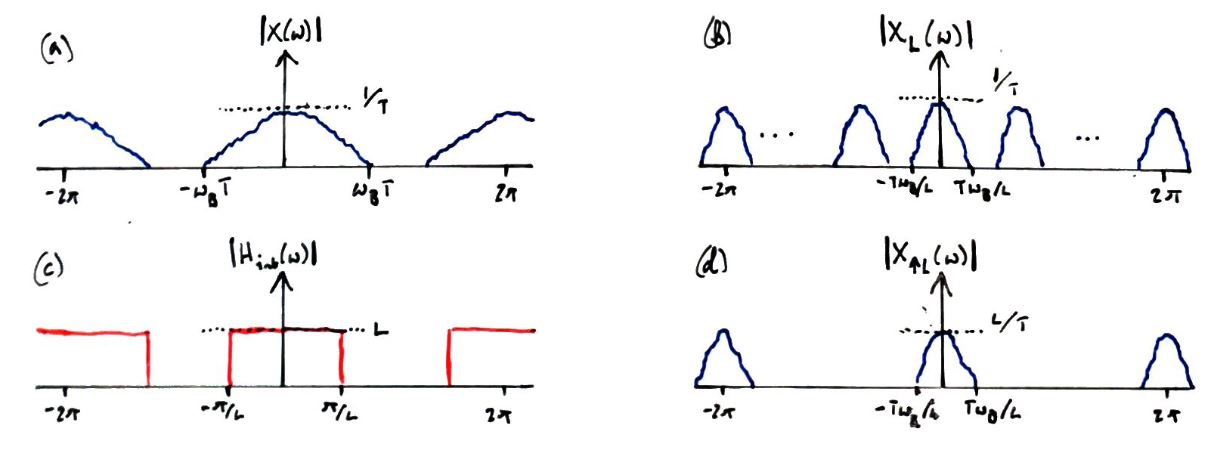
\includegraphics[width=\textwidth]{images/lecture_14_upsample.JPG}
  \caption{The DTFT of the original signal acquired at a sampling period of $T$
    (pane (a)) is upsampled by a factor of $L$ in pane (b), resulting in a scaling
    of the band-limit to $T\omega_B/L$ and a squeezing of periodic copies on
    the frequency axis such that there are $N$ copies in a $2\pi$ range.
    Use of the low-pass interpolation filter (pane (c)) then carves out
    copies such that the DTFT of the upsampled signal remains (pane (d)).
  }
  \label{fig::lecture_14_upsample}
\end{figure}
%
Upsampling is comparatively simpler than downsampling since we can't alias the
signal by upsampling. The original signal may have aliasing if it was
sampled below the Nyquist rate, and this is something that can't be rectified
by upsampling.
